{
{\sffamily Dette afsnit vil præsentere vores resultater fra
eksperimentet, hvor vi har brugt den udvidede metode, til at vurdere
regionerne. Da eksperimentet blev kørt, har vi sat opløsningen på
regionernes approksimation med et gitter for højt, hvilket er resulteret
i, at kørslen ikke er kommet igennem hele vores datasæt.
}

\subsection{Reduceret datasæt}
Kørslen har nået at analysere $608$ malerier, men som vist herunder i
tabel \ref{ud_tabel_fjern_detaljer}, har vi kun $524$ brugbare
resultater, når vi har fjernet de billeder, som ikke er hele malerier.
Dette svarer til en nedgang på $13.82\%$.

\begin{table}[H]
    \centering
    \begin{tabular}{r@{\ \ }p{12em}r|r@{.}l}
            & Analyserede malerier & $608$ & $100$ & $00\%$   \\
        $-$ & Udsnit af malerier   &  $84$ &  $13$ & $82\%$   \\\hline
            & Resultater           & $524$ &  $86$ & $18\%$
    \end{tabular}
    \caption[]{Udregning af brugbare resultater fra udvidet kørsel.}
    \label{ud_tabel_fjern_detaljer}
\end{table}

Dette svarer til $\mathsf{3.65\%}$ af de brugbare resultater fra den
naive kørsel. Vores datasæt bliver gennemgået alfabetisk efter
kunstnerens efternavn, så vi har kun resultater fra kunstnere med
efternavn startende med 'A' og 'B'.

At vi kun har et undersæt af malerierne gør, at vi bliver nødt til at se
på hvilke tidsperioder og nationaliteter vi har repræsenteret.

\begin{figure}[!h]
    \centering
    \subfloat[Årstal]{
    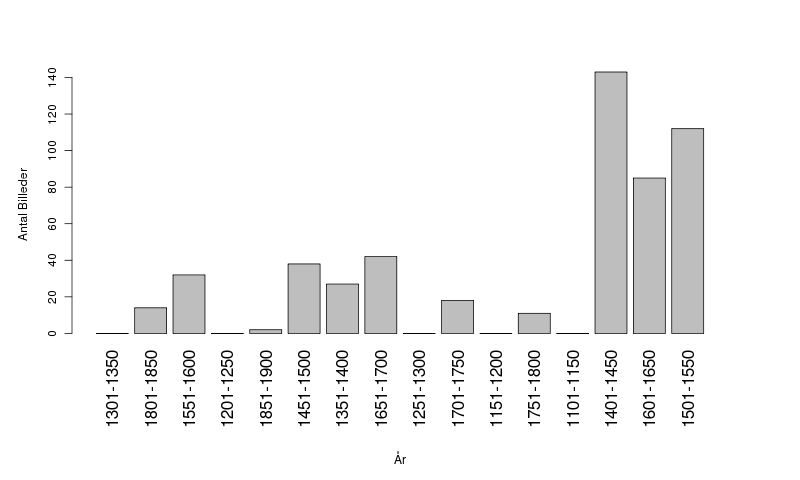
\includegraphics[angle=-90,width=0.42\textwidth]{afsnit/resultater/billeder/year}
        \label{ud_year}}\hspace{1em}
    \subfloat[Nationalitet]{
        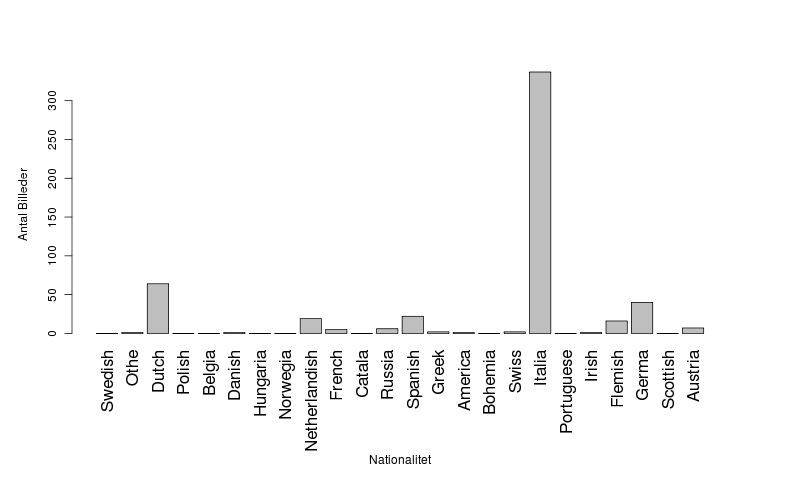
\includegraphics[angle=-90,width=0.42\textwidth]{afsnit/resultater/billeder/nation}
        \label{ud_nation}}
    \caption[]{Maleriernes årstal og nationalitet.}
    \label{ud_year_nation}
\end{figure}

\subsection{Håndtering af systematisk fejl}
Selvom denne analyse også har brugt den fejlbehæftede metode, til
udtrækning af regioner, så sorteres duplikater fra, når vi approksimerer
en region. Vi har gemt farven, som en region er blevet tildelt af
floodfill, og hvis denne farve ikke er at finde i regionens begrænsende
rektangel, betyder det, at regionen er blevet malet over senere. Vi
smider derfor denne region væk.

Den udvidede metode indeholder derfor ingen duplikater, men resultaterne
er ikke direkte sammenlignelige med dem fra den naive kørsel.

\subsection{Resultater}
Udregningen i tabel \ref{ud_tabel_fordeling} redegør for, hvor mange af
de brugbare resultater, der har mindst en region liggende i det gyldne
snit. Vi ser at der i $87.02\%$ af malerierne, er blevet fundet regioner
i det gyldne snit, og vi kan derfor ikke afvise hypotese
\ref{hypo_binaer}.

\begin{table}[H]
    \centering
    \begin{tabular}{r@{\ \ }p{12em}r|r@{.}l}
            & Positive resultater   & $456$ &  $87$ & $02\%$ \\
        $+$ & Negative resultater   &  $68$ &  $12$ & $98\%$ \\\hline
            & Resultater i alt      & $524$ & $100$ & $00\%$
    \end{tabular}
    \caption[]{Et positivt resultat beskriver et maleri hvori der er
    fundet mindst en region i det gyldne snit, ved brug af den udvidede
    vurdering af regioner.}
    \label{ud_tabel_fordeling}
\end{table}

Fordelingen af regioner, over de fire gyldne snit i malerierne, ses i
tabel \ref{ud_tabel_fire_snit}. Intet af de fire snit afviger med
mere end $10\%$ fra et andet, og vi kan således ikke afvise hypotese
\ref{hypo_fire_g_snit}.

\begin{table}[H]
    \centering
    \begin{tabular}{r@{\ \ }p{12em}r|r@{.}l}
            & Regioner i snit 0   &  $405$ &  $22$ & $29\%$ \\
        $+$ & Regioner i snit 1   &  $421$ &  $23$ & $17\%$ \\
        $+$ & Regioner i snit 2   &  $499$ &  $27$ & $46\%$ \\
        $+$ & Regioner i snit 3   &  $492$ &  $27$ & $08\%$ \\\hline
            & Regioner i alt      & $1817$ & $100$ & $00\%$
    \end{tabular}
    \caption[]{Forholdet mellem de interessante regioner fundet i de
    fire gyldne snit ved udvidet vurdering.}
    \label{ud_tabel_fire_snit}
\end{table}

\subsubsection{Antallet af fundne regioner over alle snit}
Analysen har fundet $17,705$ regioner over alle snit i malerierne, med
middelværdi $\mu = 33.79$ og standardafgivelse $\sigma = 18.58$.
Antallet af fundne regioner i malerierne er illustreret i figur
\ref{ud_graf_total_regions}. I figur \ref{ud_qq_total_regions} er vist
et QQ-plot, som viser hvorvidt vores data er normalfordelt. Dette er
tilfældet, hvis punkterne følger diagonalen i grafen. Vi ser, at de
observerede data følger linjen nogenlunde, men har et udsving nederst
til venstre, hvilket antyder at fordelingen er lidt skæv. Vi har i figur
\ref{ud_hist_total_regions} sammenlignet et histogram over de
observerede værdier, med tæthedsfunktionen for normalfordelingen $X \sim
N(\mu = 33.79, \sigma^2 = 345.22)$. De observerede værdier, følger dog
ikke de teoretiske værdier særlig pænt, og kun få steder falder de
teoretiske værdier inden for det observerede interval, hvorfor vi ikke
kan komme frem til et troværdigt konfidensinterval.

Med et større antal fundne regioner, kunne vi meget vel komme tættere på
en normalfordeling, og vi kunne da udtale os mere sikkert, om det
forventede antal fundne regioner i et arbitrært billede.

\begin{figure}[!h]
    \centering
    \subfloat[]{
        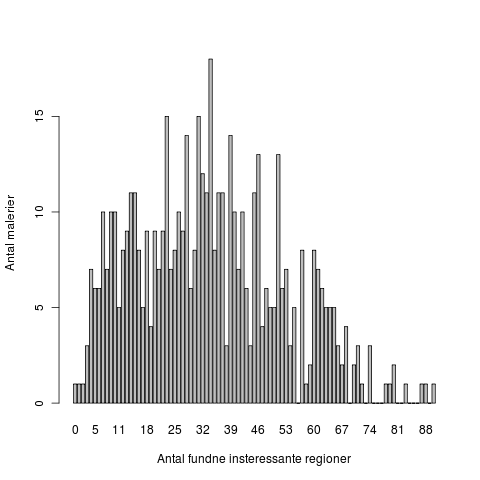
\includegraphics[width=0.49\textwidth]{afsnit/resultater/billeder/exp_totalregions}
        \label{ud_graf_total_regions}
    }
    \subfloat[]{
        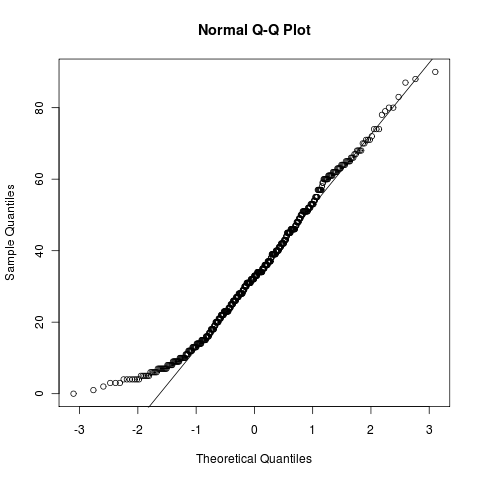
\includegraphics[width=0.49\textwidth]{afsnit/resultater/billeder/qq_exp_totalregions}
        \label{ud_qq_total_regions}
    }\\
    \subfloat[]{
        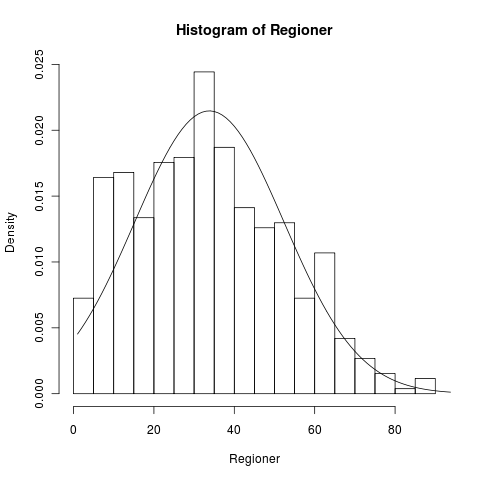
\includegraphics[width=0.62\textwidth]{afsnit/resultater/billeder/hist_exp_totalregions}
        \label{ud_hist_total_regions}
    }
    \caption[]{Fordelingen af fundne regioner på malerier ved udvidet
    vurdering.
    \textbf{\ref{ud_graf_total_regions}:} Fordelingen af de fundne
    regioner.
    \textbf{\ref{ud_qq_total_regions}:} QQ-plot, som viser at vi er tæt
    på at have en normalfordeling med den teoretiske fordeling $X \sim N(\mu,
    \sigma^2)$.
    \textbf{\ref{ud_hist_total_regions}:} Histrogram med
    tæthedsfunktionen for normalfordeling, hvor $\mu = 33.79$ og
    $\sigma^2 = 345.22$.
    }
    \label{ud_total_regions_plots}
\end{figure}

\subsubsection{Spacer}

% Spacer! Ikke over denne linje HAHAHA

I graf \ref{antal_regioner_vertikale_cut_udvidet} er der afbilledet,
antale sammelet regioner i de 20 vertikale snit for helle datasættet.
Som man kan se er der fundet makant flere regioner i de to snit som
ligger tættest på miden, og færest ud i kanterne. 

\begin{figure}[h!]
	\begin{center}
		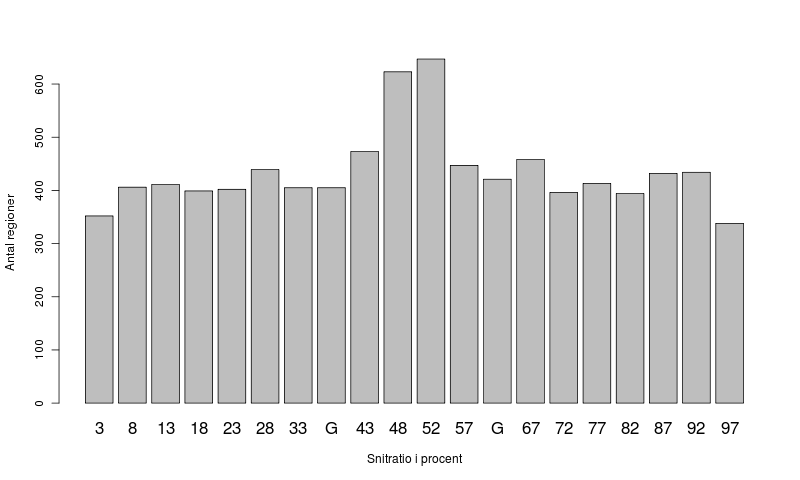
\includegraphics[width=0.9\textwidth]{afsnit/resultater/billeder/cut0cut1eatsperratioU.png}
	\end{center}
	\caption{Antal regioner i hvert af de 20 vertikale snit}
	\label{antal_regioner_vertikale_cut_udvidet}
\end{figure}

I graf \ref{antal_regioner_horisontale_cut_udvidet} er der samme
afbildning lavet, bare i det hoisontale plan, med venster side af grafen
svare til toppen af billedet. I denne graf er det 72,82 som peaker. Fra
52 og ned af, falder antal regioner gradvis. hvor i mod fra 52 og op gå
grafen lidt op og lidt ned. Kanterne er igen klart de lavest i grafen.

\begin{figure}[h!]
	\begin{center}
		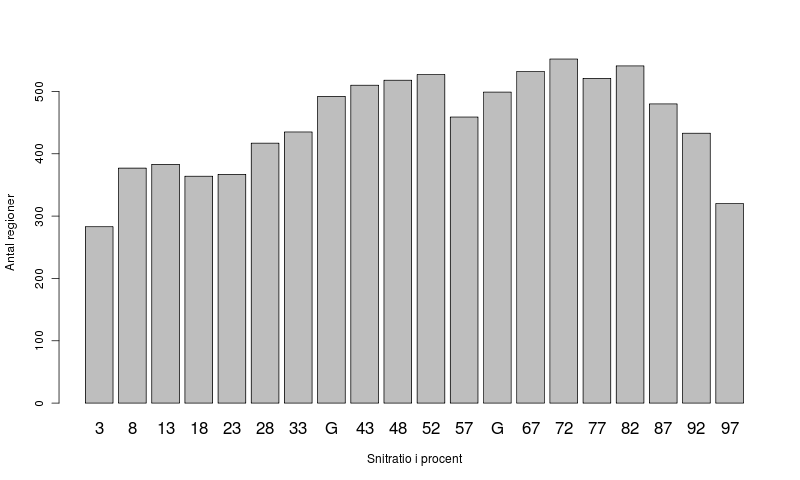
\includegraphics[width=0.9\textwidth]{afsnit/resultater/billeder/cut2cut3eatsperratioU.png}
	\end{center}
	\caption{Antal regioner i hvert af de 20 horisontale snit, hvor venstre side af grafen repræsentere øverst del af malerierne}
	\label{antal_regioner_horisontale_cut_udvidet}
\end{figure}

Ud fra disse observationer kan vi konkludere at der ikke er flere
regioner i det gyldne snit, en midden af billedet, og kan derfor
forkaste hypotese \ref{hypo_alle_andre_snit} og \ref{hypo_midten}.

I graf \ref{G_vs_to_trejedele_udvidet}, er de fire gyldne snit, samt
$\frac{2}{3}$ representeret. Som man kan se der ikke nogen entydighed på
hvad for et ration, der er dominerne, så vi kan forkaste hyptese
\ref{hypo_to_tredjedele}.

\begin{figure}[h!]
	\begin{center}
		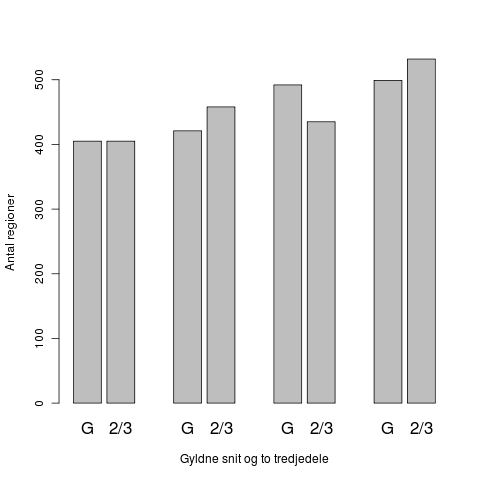
\includegraphics[width=0.6\textwidth]{afsnit/resultater/billeder/G_vs_to_tredjedeleU.png}
	\end{center}
	\caption{Procent vis antal regioner i de fire gyldne snit og deres tilhørene $\frac{2}{3}$ snit}
	\label{G_vs_to_trejedele_udvidet}
\end{figure}

I graferne \ref{udvidet_year}, kan man se de 4 gyldnes snit, og hvor
mange regioner der er fundet i gennemsnit per billedet i alle
tidsperioder. Tidsperioder hvor ingen malerier er analyseret, er ikke
taget med. Som man kan se i tidsperioden 1401-1450 for de fire snit,
bliver der fundet ca 0.2 flere regioner i gennemsnit. Da den
gennemsnit maksimale fundene regioner ligger og svinger mellem 1.1 og
1.5. Må der være mere en ti procent flere regioner i nogle tidsperioder
en andre. Så hypotese \ref{hypo_tid} kan forkastes. 

\begin{figure}[!h]
    \centering
    	\subfloat[Det gyldne snit 0.]{
	       	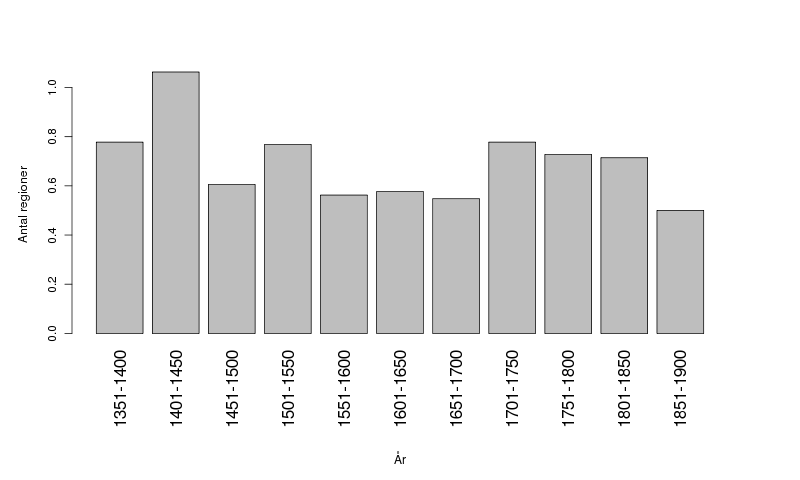
\includegraphics[angle=-90,width=0.42\textwidth]{afsnit/resultater/billeder/yearcut0U.png}
	       	\label{udvidet_year_cut0}}\hspace{1em}
		\subfloat[Det gyldne snit 1.]{
	       	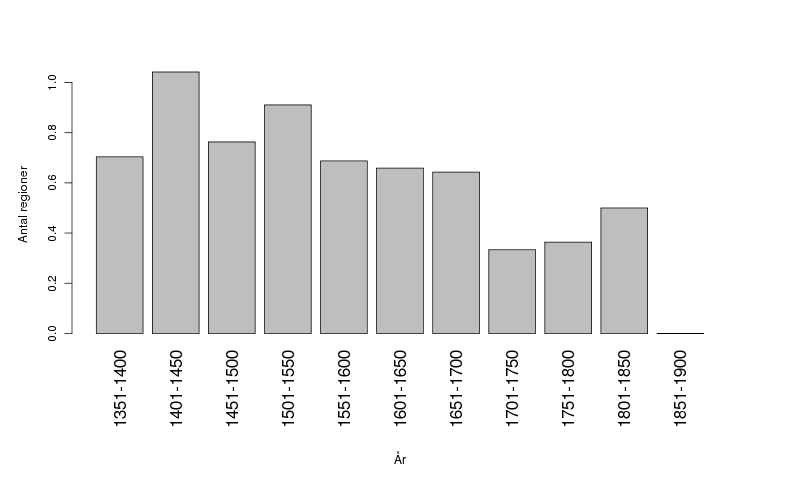
\includegraphics[angle=-90,width=0.42\textwidth]{afsnit/resultater/billeder/yearcut1U.png}
	       	\label{udvidet_year_cut1}}\hspace{1em}\\
		\subfloat[Det gyldne snit 2.]{
	       	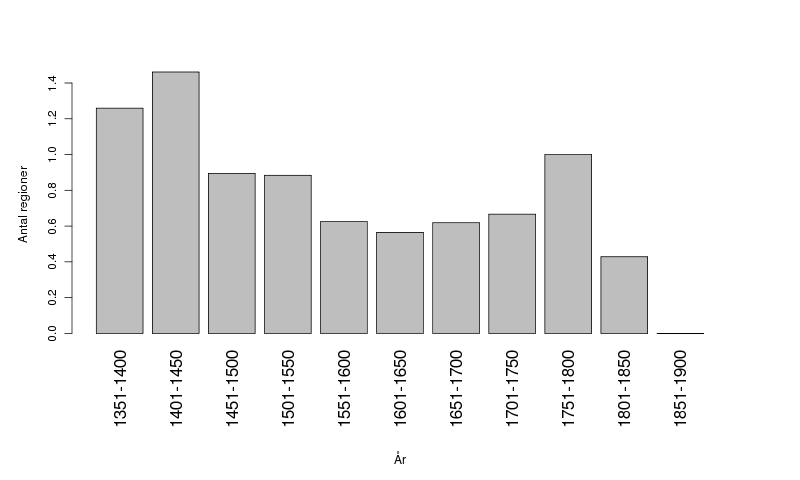
\includegraphics[angle=-90,width=0.42\textwidth]{afsnit/resultater/billeder/yearcut2U.png}
	       	\label{udvidet_year_cut2}}\hspace{1em}
		\subfloat[Det gyldne snit 3.]{
	       	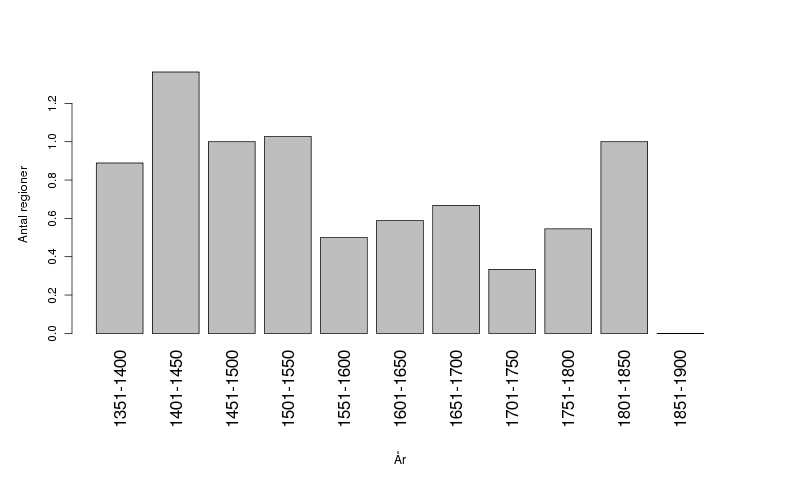
\includegraphics[angle=-90,width=0.42\textwidth]{afsnit/resultater/billeder/yearcut3U.png}
	       	\label{udvidet_year_cut3}}\hspace{1em}
       \caption[]{Fire grafer over antal regioner fundet i vær sig
       tidsperiode. Vær graf repræsentere vær deres snit. Y aksen er det
       gemmesnitlige antal fundene regioner i snittet.}
     \label{udvidet_year}
\end{figure}
I grafene \ref{udvidet_nation}, kan 
\begin{figure}[!h]
    \centering
    	\subfloat[Det gyldne snit 0.]{
	       	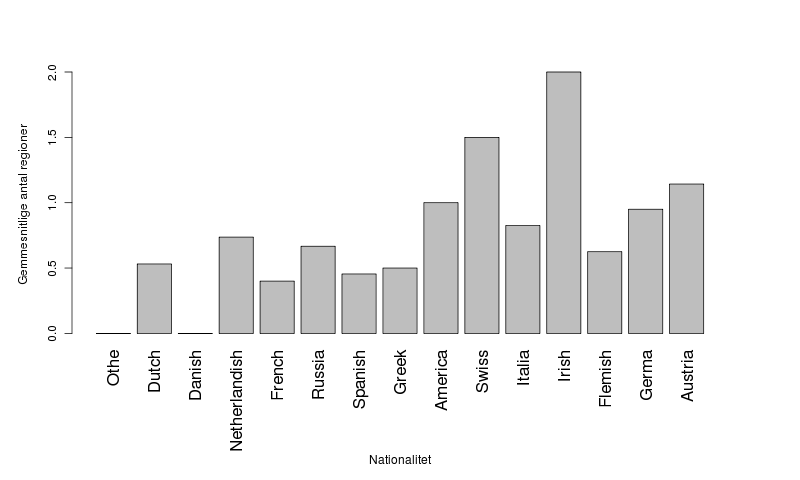
\includegraphics[angle=-90,width=0.42\textwidth]{afsnit/resultater/billeder/nationcut0U.png}
	       	\label{udvidet_nation_cut0}}\hspace{1em}
		\subfloat[Det gyldne snit 1.]{
	       	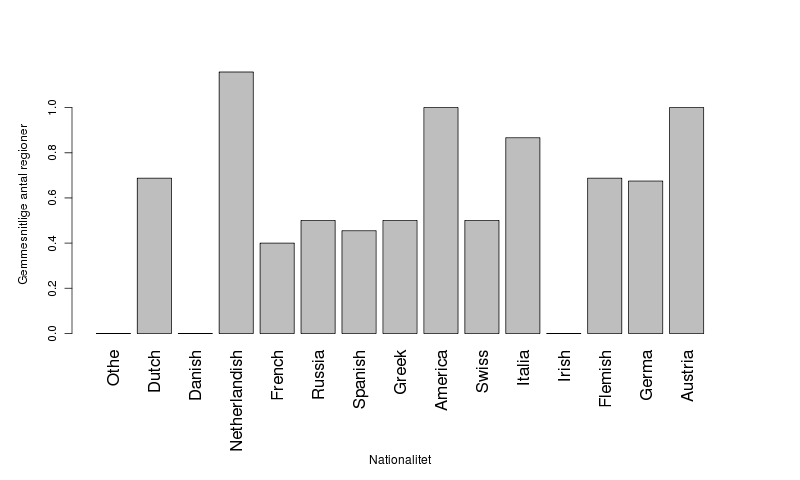
\includegraphics[angle=-90,width=0.42\textwidth]{afsnit/resultater/billeder/nationcut1U.png}
	       	\label{udvidet_nation_cut1}}\hspace{1em}\\
		\subfloat[Det gyldne snit 2.]{
	       	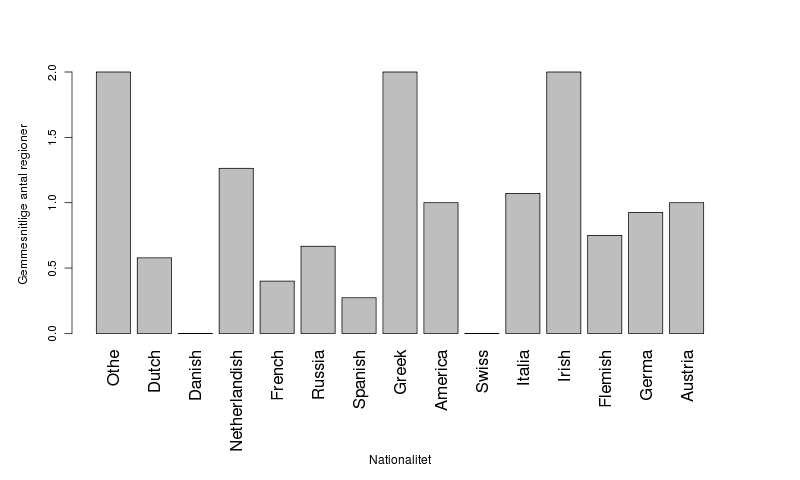
\includegraphics[angle=-90,width=0.42\textwidth]{afsnit/resultater/billeder/nationcut2U.png}
	       	\label{udvidet_nation_cut2}}\hspace{1em}
		\subfloat[Det gyldne snit 3.]{
	       	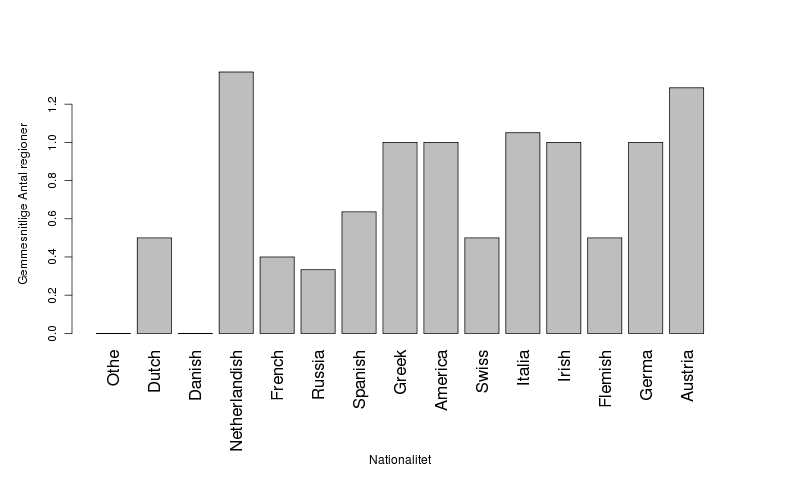
\includegraphics[angle=-90,width=0.42\textwidth]{afsnit/resultater/billeder/nationcut3U.png}
	       	\label{udvidet_nation_cut3}}\hspace{1em}
       \caption[]{Fire grafer over antal regioner fundet i vær sig
       nationalitet. Vær graf repræsentere vær deres snit. Y aksen er det
       gemmesnitlige antal fundene regioner i snittet.}
     \label{udvidet_nation}
\end{figure}



\begin{table}[!h]
    \centering
    \begin{tabular}{|l|c|c|}
        \hline
            & Afvist & Ikke afvist  \\\hline
        1   &            & \checkmark   \\\hline
        2   &            & \checkmark   \\\hline
        3   & \checkmark$^{\textrm{*}}$ &              \\\hline
        4   & \checkmark &              \\\hline
        5   & \checkmark &    	\\\hline
        6   & \checkmark &              \\\hline
        7   & \checkmark &              \\\hline
        8   &            &              \\\hline
        9   &            & 	\\\hline
    \end{tabular}
    \caption[]{Hypoteser i forhold til den udvidet kørsel.
    $^{\textrm{*}}$Jvf. udregning \ref{tabel_real_dimensions}.
    }
    \label{hypoteser_udvidet}
\end{table}

} % Eh eh eh. Nallerne væk!

% vim: set tw=72 spell spelllang=da:
